\input{./_path-to-root.ltx}
\documentclass[\PathToRoot/\ProjectName]{subfiles}
\whenstandalone{\externaldocument{\PathToRoot/\ProjectName}}

\begin{document}

\begin{figure}[htb] 
  \centering
  \caption{Wealth distribution comparison without splurge factor}
  \whenintegrated{\label{fig:LorenzPtsSplZero}} 
  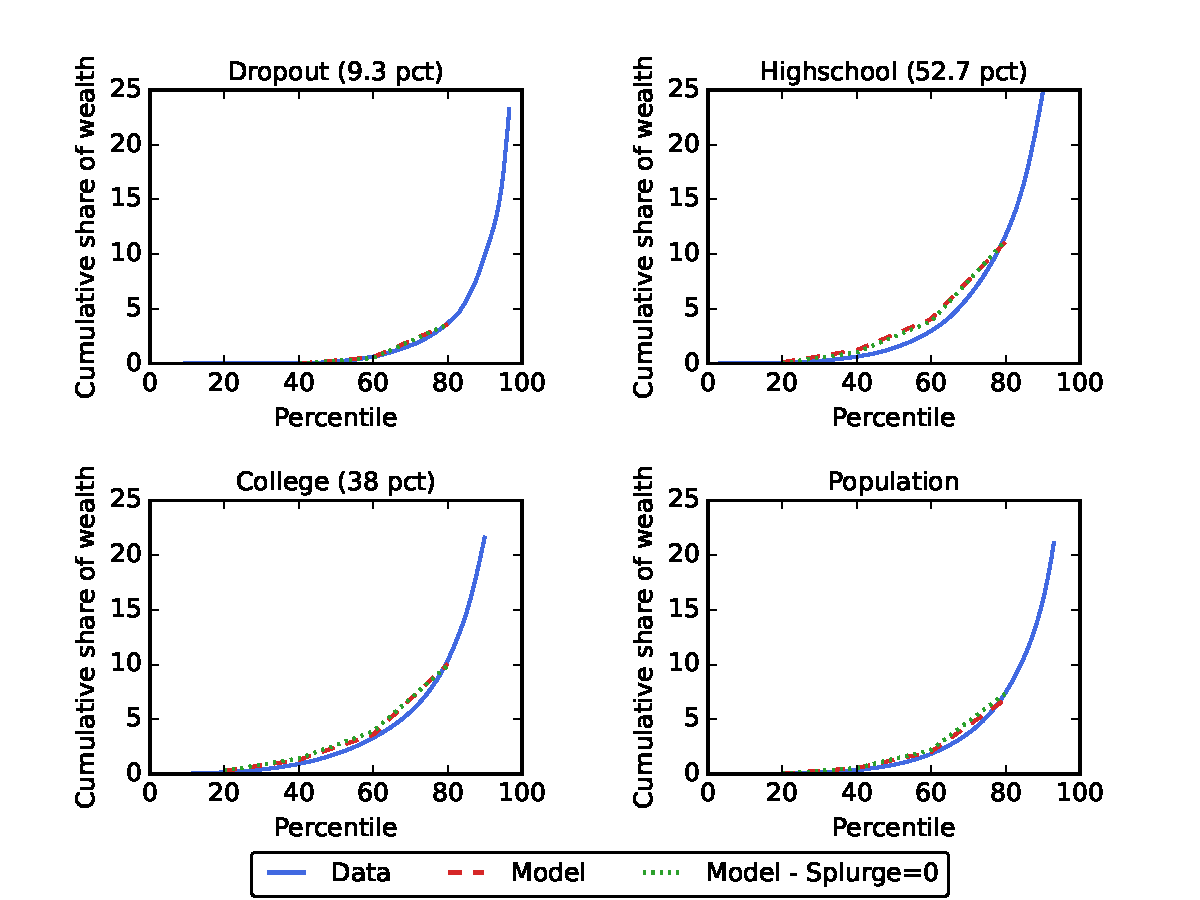
\includegraphics[width=.9\textwidth]{\PathToRoot/images/LorenzPoints_CRRA_2.0_R_1.01_wSplZero}

  \medskip
  \noindent\parbox{\textwidth}{\footnotesize
    \textbf{Note}: This figure shows liquid wealth distributions in the model without splurge factor (Appendix~\ref{app:Model-without-splurge}).
    The no-splurge model requires wider discount factor distributions to achieve similar empirical fit,
    resulting in more unequal wealth distribution compared to the baseline model and 2004 SCF data.
    The model generates higher inequality particularly for the College group and highest wealth quartile,
    as shown in Table~\ref{tab:nonTargetedMoments-wSplZero}. While performance remains reasonable,
    this validates the empirical advantage of including the splurge factor for matching both spending
    dynamics and wealth distribution simultaneously.
  }
\end{figure}

\vspace{0.5em}

% Smart bibliography: Only include bibliography if standalone AND has citations
\smartbib

\end{document}
